% % ExVA/Lego/256:     u4108 -> lego_random_exr
% %       150k:   24.00 & 0.88 & 0.101 & 0.207 & 150k & 256px & 11h30m
% %       80k:    23.76 & 0.87 & 0.117 & 0.215 & 80k & 256px & 5h

% \begingroup
% \begin{figure}[!htb]
%     % \setArraystrech{1.5}
%     \centering
%     \setlength\tabcolsep{2pt}
%     \begin{tabular*}{\textwidth}{ c c c c }
%           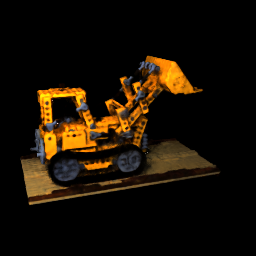
\includegraphics[width=0.19\textwidth]{figures/results/arb_set/lego7_exva_150k.png}
%         & \includegraphics[width=0.19\textwidth]{figures/results/arb_set/lego7_exva_normal_150k.png}
%         & \includegraphics[width=0.19\textwidth]{figures/results/arb_set/lego7_exva_roughness_150k.png}
%         & \includegraphics[width=0.19\textwidth]{figures/results/arb_set/lego7_exva_depth_150k.png} \\
        
%           \includegraphics[width=0.19\textwidth]{figures/results/arb_set/lego7_exva_voxel_4k.png}
%         & \includegraphics[width=0.19\textwidth]{figures/results/arb_set/lego7_exva_voxel_18k.png}
%         & \includegraphics[width=0.19\textwidth]{figures/results/arb_set/lego7_exva_voxel_45k.png}
%         & \includegraphics[width=0.19\textwidth]{figures/results/arb_set/lego7_exva_voxel_150k.png}
        

%     \end{tabular*}
%     \caption{\im{Fix width and add description!}}
%     \label{tab:arb_maps}
% \end{figure}
% \endgroup